% Fundamentals of Microcontrollers Manual
% 
% Manual to accompany the class lectures and lab
%
% Seth McNeill
% Started 2021 November 16

\documentclass[12pt,oneside]{book}
\usepackage{datetime}  % for automated current date on the document
\setcounter{secnumdepth}{3}  % to make subsubsections numbered
\usepackage{amsmath}  % for aligned equations and such
\usepackage{xcolor}  % to color text
\usepackage[pdftex]{graphicx} % for includegraphics?
\usepackage{siunitx}  % for aligning tables by decimal point
\usepackage{pdfpages}  % to include PDF files in the document

% For creating nice addition figures
% based on https://tex.stackexchange.com/a/96764
\usepackage{cancel}
\usepackage{tikz}
\usetikzlibrary{matrix}
\newcommand{\addend}{\text{\textsl{\color{gray}{Addend}}}}
\newcommand{\augend}{\text{\textsl{\color{gray}{Augend}}}}
\newcommand{\sumOut}{\text{\textsl{\color{gray}{Sum}}}}
% end addition figure requirements
\usepackage{hyperref}  % for URL hyperlinks

\hypersetup{
colorlinks,
citecolor=black,
filecolor=black,
linkcolor=blue,
urlcolor=blue
}

% for automated current date on the document
\newdateformat{myDate}{\THEYEAR{ }\monthname[\THEMONTH] \twodigit{\THEDAY}}

% Referencing commands 
\newcommand{\chaplabel}[1]{\label{chap:#1}}
\newcommand{\chapref}[1]{Chapter~\ref{chap:#1}}
\newcommand{\seclabel}[1]{\label{sec:#1}}
\newcommand{\secref}[1]{Section~\ref{sec:#1}}

\title{Fundamentals of Applied Microcontrollers Manual}
\author{Seth McNeill}
\date{Edition 0.01 \\ \myDate\today}

\begin{document}
	\maketitle

	\tableofcontents

	% include chapters here
	\chapter{Introduction}
\chaplabel{intro}

\section{Introduction}
This book is the accompanying text to a class introducing microcontrollers
to upper division, non-electrical engineering undergraduate students who 
have taken some C programming.

The accompanying laboratory manual is located 
\href{https://github.com/semcneil/Fundamentals-of-Microcontrollers-Laboratories}{here}.

\section{License}
This code is released under a Creative Commons Attribution license.
The full text of the license is available at the following link.

\href{https://creativecommons.org/licenses/by/4.0/}{https://creativecommons.org/licenses/by/4.0/}

Users of this code should attribute the work to this
project by displaying a notice stating their product contains code
and/or text from the Fundamentals of Microcontrollers Project and/or linking to\\
https://github.com/semcneil/Fundamentals-of-Microcontrollers-Laboratories.
	\chapter{Number Systems}
\chaplabel{numbers}

This chapter introduces the concepts of different numbering systems that
are relevant to microcontrollers.
	\chapter{Boolean Logic}
\chaplabel{logic}

This introduces some basic Boolean logic including gates and Boolean algebra.

\begin{figure}[!htb]
	\centering
	\includegraphics[scale=0.7]{logic/NAND.eps}
	\caption{The NAND gate outputs NOT(A AND B).}
	\label{fig:nand}
  \end{figure} 
	\chapter{Arduino Startup}
\chaplabel{arduino}

\section{Introduction}
This chapter gets students started with the Arduino IDE.

\section{Installing the IDE}
These directions assume that you are using the lab computers and One Drive.
\begin{enumerate}
	\item Go to software download page: \href{https://www.arduino.cc/en/software}{https://www.arduino.cc/en/software}
	\item Download the Windows ZIP file (not the first link or the app)
	\item Open the zip file and copy the folder inside (arduino-1.8.19 as of this writing) into your One Drive folder. This may take a while. If you are on your own computer, you can use any of the programs.
	\item Once that transfer finishes, go into the folder and run arduino.exe. Windows will try to save you, but if you click More Info you can click Run Anyway.
	\item Windows Defender Firewall will also complain. Uncheck the box that is checked and/or click Cancel.
	\item It should load up with a window that looks like Figure \ref{fig:emptysketch}.
	\item In order to get it to connect correctly to your board, you need to install the Arduino Nano Connect RP2040 board.
	\begin{enumerate}
		\item Navigate to Tools$\rightarrow$Board: "Arduino Uno" (or similar)$\rightarrow$Boards Manager
		\item It should load as shown in Figure \ref{fig:boardsManager}.
		\item In the search bar, type "arduino nano connect" (without the quotes)
		\item The first item should be Arduino Mbed OS Nano Boards and should list the Arduino Nano RP2040 Connect.
		\item Move your cursor over it and it should show an Install button. Click it to install the board library.
		\item Wait for it to finish.
		\item While you are waiting, plug your Nano Connect into your computer and let it install it.
		\item As it finished, I received a User Account Control warning asking if I wanted to let dpinst-amd64.exe make changes to my device. I said yes.
		\item Next it asked me if I wanted to install Arduino Universal Serial Bus devices. Again, click to Install.
		\item It popped up again and I clicked Install again. Now it should say that the Arduino Mbed OS Nano Boards has been installed.
		\item Close the Boards Manager.
	\end{enumerate}
	\item Now go to Files$\rightarrow$Examples$\rightarrow$01.Basics$\rightarrow$Blink.
	\item This will open another window with the Blink program.
	\item Go to Tools$\rightarrow$Board$\rightarrow$Arduino Mbed OS Nano Boards and select the Arduino Nano RP2040 Connect
	\item Go to Tools$\rightarrow$Port and select the COM that isn't COM1 (mine showed up as COM5)
	\item Click the right arrow under the word edit in the menu to Uplaod the sketch to the Arduino board.
	\item It should say "Compiling sketch..." in the lower left and show a progress bar on the lower right.
	\item Then it should switch to Uploading... and finally Done Uploading.
	\item An orange light near the USB port on your board should be blinking.
	\item Congratulations! You have programmed your board!
	\item Now look in the program for the two delay statements. Try changing the values inside the parentheses and re-uploading it. Does the blinking change?
	\item In order to save files and have it portable, you need to change the directory where the Arduino IDE stores it's sketchbooks
	\begin{enumerate}
		\item Go to File$\rightarrow$Preferences
		\item Change the Sketchbook location to your OneDrive and a folder named arduino (lowercase is good)
		\item My OneDrive was in C:\textbackslash Users\textbackslash mcneils2\textbackslash OneDrive - Embry-Riddle Aeronautical University\textbackslash arduino
	\end{enumerate}
\end{enumerate}

\begin{figure}[!htb]
	\centering
	\includegraphics[scale=1.0]{arduinoStart/emptysketch.PNG}
	\caption{This is what the Arduino IDE should load up to.}
	\label{fig:emptysketch}
\end{figure} 

\begin{figure}[!htb]
	\centering
	\includegraphics[scale=1.0]{arduinoStart/BoardsManager.PNG}
	\caption{This what the Boards Manager loads up to.}
	\label{fig:boardsManager}
\end{figure} 

	%\chapter{Buttons and Serial Communications}
\chaplabel{buttons}

\section{Introduction}
This chapter introduces students to using buttons and serial communications.

\section{Buttons}

A typical button circuit is shown in Figure \ref{fig:buttonPullup}. The input is high until the button is pressed.
Unfortunately, being mechanical, buttons do not always create nice, clean switched inputs. Maxim Integrated has a 
\href{https://www.maximintegrated.com/en/design/technical-documents/app-notes/2/287.html}{nice paper} on the topic
advertizing their devices to solve the problem. However, if we don't have the option of adding their hardware, some 
work can be done in software to debounce an input. As Maxim mentions, software debouncing is not free. It does incur
some overhead so you probably do not want to do it for many inputs. Am example of software debouncing is in 
Listing \ref{lst:debounce}.

\begin{lstlisting}[language=C++, caption={This is the Arduino example of software debouncing.},label={lst:debounce}]
	/*
	Debounce
  
	Each time the input pin goes from LOW to HIGH (e.g. because of a push-button
	press), the output pin is toggled from LOW to HIGH or HIGH to LOW. There's a
	minimum delay between toggles to debounce the circuit (i.e. to ignore noise).
  
	The circuit:
	- LED attached from pin 13 to ground through 220 ohm resistor
	- pushbutton attached from pin 2 to +5V
	- 10 kilohm resistor attached from pin 2 to ground
  
	- Note: On most Arduino boards, there is already an LED on the board connected
	  to pin 13, so you don't need any extra components for this example.
  
	created 21 Nov 2006
	by David A. Mellis
	modified 30 Aug 2011
	by Limor Fried
	modified 28 Dec 2012
	by Mike Walters
	modified 30 Aug 2016
	by Arturo Guadalupi
  
	This example code is in the public domain.
  
	https://www.arduino.cc/en/Tutorial/BuiltInExamples/Debounce
  */
  
  // constants won't change. They're used here to set pin numbers:
  const int buttonPin = 9;    // the number of the pushbutton pin
  const int ledPin = 13;      // the number of the LED pin
  
  // Variables will change:
  int ledState = LOW;         // the current state of the output pin
  int buttonState;             // the current reading from the input pin
  int lastButtonState = LOW;   // the previous reading from the input pin
  
  // the following variables are unsigned longs because the time, measured in
  // milliseconds, will quickly become a bigger number than can be stored in an int.
  unsigned long lastDebounceTime = 0;  // the last time the output pin was toggled
  unsigned long debounceDelay = 50;    // the debounce time; increase if the output flickers
  
  void setup() {
	Serial.begin(115200);
	while(!Serial) delay(10);
	Serial.println("Starting...");
	
	pinMode(buttonPin, INPUT);
	pinMode(ledPin, OUTPUT);
  
	// set initial LED state
	digitalWrite(ledPin, ledState);
  }
  
  void loop() {
	// read the state of the switch into a local variable:
	int reading = digitalRead(buttonPin);
  
	// check to see if you just pressed the button
	// (i.e. the input went from LOW to HIGH), and you've waited long enough
	// since the last press to ignore any noise:
  
	// If the switch changed, due to noise or pressing:
	if (reading != lastButtonState) {
	  // reset the debouncing timer
	  lastDebounceTime = millis();
	}
  
	if ((millis() - lastDebounceTime) > debounceDelay) {
	  // whatever the reading is at, it's been there for longer than the debounce
	  // delay, so take it as the actual current state:
  
	  // if the button state has changed:
	  if (reading != buttonState) {
		buttonState = reading;
  
		// only toggle the LED if the new button state is HIGH
		if (buttonState == HIGH) {
		  ledState = !ledState;
		}
	  }
	}
  
	// set the LED:
	digitalWrite(ledPin, ledState);
  
	// save the reading. Next time through the loop, it'll be the lastButtonState:
	lastButtonState = reading;
  
  }
\end{lstlisting}

\begin{figure}[!htb]
	\centering
	\includegraphics{buttonSerial/button1.eps}
	\label{fig:buttonPullup}
	\caption{This is a typical button input circuit.}
\end{figure}

\begin{figure}[!htb]
	\centering
	\includegraphics[scale=0.5]{buttonSerial/debounce.eps}
	\label{fig:buttonDebounce}
	\caption{This is an example of what the output signal from a button with the circuit in Figure \ref{fig:buttonPullup} could look like.}
\end{figure}


\section{Types of Serial}

\begin{figure}[!htb]
	% Serial
	\centering
	\begin{tikzpicture}
		% BLOCKS
		\draw[thick] (0,0) rectangle (4,4) node (dev1) [pos=0.5] {Device 1};
		\draw[thick] (8,0) rectangle (12,4) node (dev2) [pos=0.5] {Device 2};
		% ARROWS	
		\draw [thick,-{latex[length=4mm, width=6mm]}] (4,2) |- node [above,pos=0.75] {01101101} (8,2) ;
	\end{tikzpicture}
	\label{fig:serial}
	\caption{Serial transfers one bit at a time.}
\end{figure}
	
	% Parallel
\begin{figure}[!htb]
	\centering
	\begin{tikzpicture}
		% BLOCKS
		\draw[thick] (0,0) rectangle (4,5) node (dev3) [pos=0.5] {Device 1};
		\draw[thick] (8,0) rectangle (12,5) node (dev4) [pos=0.5] {Device 2};
		% ARROWS	
		\draw [thick,-{latex[length=4mm, width=6mm]}] (4,4.25) |- node [above,pos=0.75] {0} (8,4.25) ;
		\draw [thick, -{latex[length=4mm, width=6mm]}] (4,3.75) |- node [above,pos=0.75] {1} (8,3.75) ;
		\draw [thick, -{latex[length=4mm, width=6mm]}] (4,3.25) |- node [above,pos=0.75] {1} (8,3.25) ;
		\draw [thick, -{latex[length=4mm, width=6mm]}] (4,2.75) |- node [above,pos=0.75] {0} (8,2.75) ;
		\draw [thick, -{latex[length=4mm, width=6mm]}] (4,2.25) |- node [above,pos=0.75] {1} (8,2.25) ;
		\draw [thick, -{latex[length=4mm, width=6mm]}] (4,1.75) |- node [above,pos=0.75] {1} (8,1.75) ;
		\draw [thick, -{latex[length=4mm, width=6mm]}] (4,1.25) |- node [above,pos=0.75] {0} (8,1.25) ;
		\draw [thick, -{latex[length=4mm, width=6mm]}] (4,0.75) |- node [above,pos=0.75] {1} (8,0.75) ;
		
	\end{tikzpicture}
	\label{fig:parallel}
	\caption{Parallel transfers multiple bits at a time.}
\end{figure}

\begin{figure}[!htb]
	% UART
	\centering
	\begin{tikzpicture}
		% BLOCKS
		\draw[thick] (0,0) rectangle (4,4) node (dev1) [pos=0.5] {Device 1};
		\draw[thick] (8,0) rectangle (12,4) node (dev2) [pos=0.5] {Device 2};
		% ARROWS	
		\draw [thick,-{latex[length=4mm, width=6mm]}] (4,2.5) node [anchor=east] {TX} -- (8,1.5) node [anchor=west] {RX} ;
		\draw [thick,{latex[length=4mm, width=6mm]}-] (4,1.5) node [anchor=east] {RX} -- (8,2.5) node [anchor=west] {TX} ;
	\end{tikzpicture}
	\label{fig:uart}
	\caption{A UART has full duplex between two entities.}
\end{figure}

\begin{figure}[!htb]
	% SPI
	\centering
	\begin{tikzpicture}
		% BLOCKS
		\draw[thick] (0,0) rectangle (4,4) node (dev1) [pos=0.5] {Controller};
		\draw[thick] (8,0) rectangle (12,4) node (dev2) [pos=0.5] {Peripheral 1};
		\draw[thick] (8, -2) rectangle (12,-6) node (dev3) [pos=0.5] {Peripheral 2};
		% ARROWS	
		\draw [thick,-{latex[length=4mm, width=6mm]}] (4,2.5) node [anchor=east] {COPI} -- (8,2.5) node [anchor=west] {COPI} ;
		\draw [thick,{latex[length=4mm, width=6mm]}-] (4,1.5) node [anchor=east] {CIPO} -- (8,1.5) node [anchor=west] {CIPO} ;
		\fill[black]  (6,1.5) circle (3pt) ;
		\draw [thick] (6,1.5) |- (8,-3.5) node [anchor=west] {CIPO} ;
		\draw [thick, -{latex[length=4mm, width=6mm]}] (7,2.5) |- (8,-2.5) node [anchor=west] {COPI} ;
		\fill[black]  (7,2.5) circle (3pt) ;
		\draw [thick,-{latex[length=4mm, width=6mm]}] (4,3.5) node [anchor=east] {CS1} |- (8,3.5) node [anchor=west] {CS} ;
		\draw [thick,-{latex[length=4mm, width=6mm]}] (4,0.5) node [anchor=east] {CS2} |- (5,0.5) |- (8,-4.5) node [anchor=west] {CS} ;
	\end{tikzpicture}
	\label{fig:spi}
	\caption{SPI allows for one (sometime more) controller and multiple peripherals.}
\end{figure}

\begin{figure}[!htb]
	% I2C
	\centering
	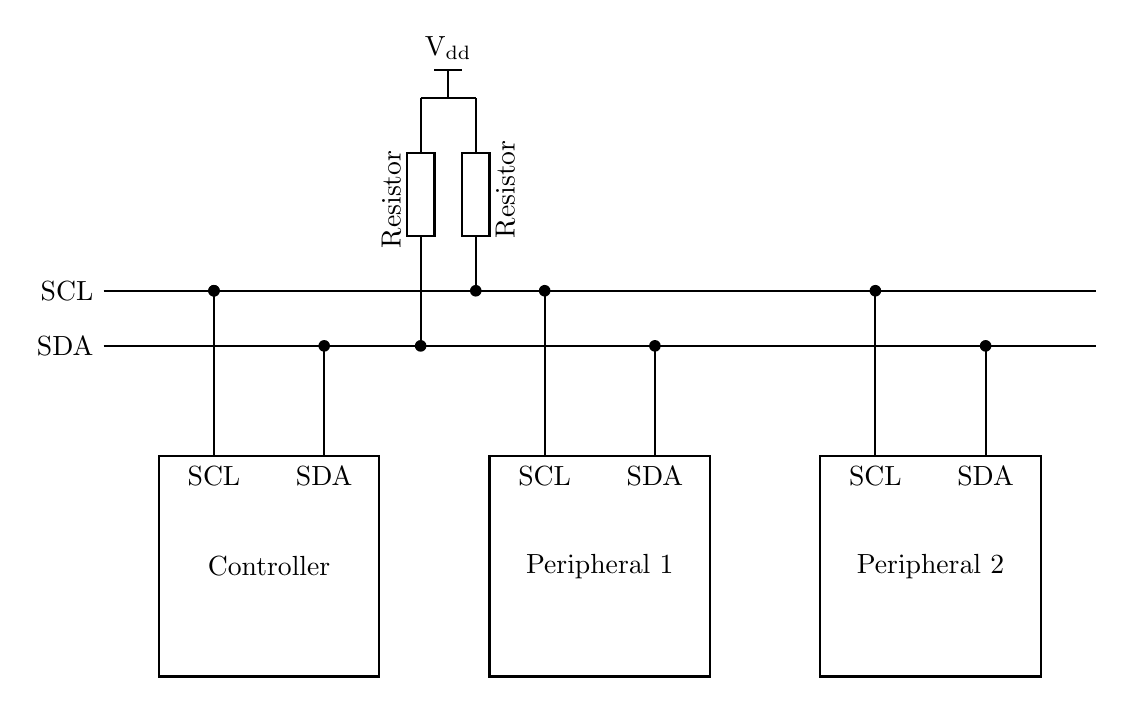
\begin{tikzpicture}[scale=0.7]
		% BLOCKS
		\draw[thick] (0,0) rectangle (4,4) node (dev1) [pos=0.5] {Controller};
		\draw[thick] (6,0) rectangle (10,4) node (dev2) [pos=0.5] {Peripheral 1};
		\draw[thick] (12, 0) rectangle (16,4) node (dev3) [pos=0.5] {Peripheral 2};
		\draw[thick] (4.5, 8) rectangle (5,9.5) node (r1) [above=2ex,pos=0.15, rotate=90] {Resistor};
		\draw[thick] (5.5, 8) rectangle (6,9.5) node (r2) [below=2ex,pos=0.85, rotate=90] {Resistor};
		
		% ARROWS	
		\draw [thick] (-1,6) node [anchor=east] {SDA} -- (17,6) ;
		\draw [thick] (-1,7) node [anchor=east] {SCL} -- (17,7)  ;
		\draw [thick] (1,4) node [anchor=north] {SCL} -- (1,7) ;
		\draw [thick] (3,4) node [anchor=north] {SDA} -- (3,6) ;
		\draw [thick] (7,4) node [anchor=north] {SCL} -- (7,7) ;
		\draw [thick] (9,4) node [anchor=north] {SDA} -- (9,6) ;
		\draw [thick] (13,4) node [anchor=north] {SCL} -- (13,7) ;
		\draw [thick] (15,4) node [anchor=north] {SDA} -- (15,6) ;
		\fill[black]  (1,7) circle (3pt) ;
		\fill[black]  (1,7) circle (3pt) ;
		\fill[black]  (7,7) circle (3pt) ;
		\fill[black]  (13,7) circle (3pt) ;
		\fill[black]  (3,6) circle (3pt) ;
		\fill[black]  (9,6) circle (3pt) ;
		\fill[black]  (15,6) circle (3pt) ;
		\draw [thick] (4.75,6)  -- (4.75,8) ;
		\fill[black]  (4.75,6) circle (3pt) ;
		\draw [thick] (5.75,7)  -- (5.75,8) ;
		\fill[black]  (5.75,7) circle (3pt) ;
		\draw [thick] (5.75,9.5)  -- (5.75,10.5) ;
		\draw [thick] (4.75,9.5)  -- (4.75,10.5) ;
		\draw [thick] (4.75,10.5)  -- (5.75,10.5) ;
		\draw [thick] (5.25,10.5)  -- (5.25,11) ;
		\draw [thick] (5,11)  -- node [above,pos=0.5] {V\textsubscript{dd}} (5.5,11) ;
	\end{tikzpicture}
	\label{fig:i2c}
	\caption{I\textsuperscript{2}C allows for multiple controllers and peripherals on the same bus.}
\end{figure}


\section{I2C}
I2C addresses for modules that are on the board or may be used with the board can be seen in Table \ref{table:i2caddresses}.

\begin{table}[!ht]
	\centering
	\begin{tabular}{l l}
		\hline
		Address (HEX) & Module \\ 
		\hline
		0x44 or 0x45 & SHT31-DIS Temperature/Humidity \\
		0x3D & 1.3" 128x64 OLED Display \\
		0x39 & APDS-9960 Light, Color, Proximity, Gesture \\
		0x77 & BME688 Temperature, Humidity, Gas \\
		0x2D, 0x53, and 0x57 & ST25DV16 Dynamic NFC/RFID Tag IC \\
		0x30 or other  & NeoKey 1x4 QT breakout board \\
		0x10 & STEMMA MiniGPS \\
		\hline
	\end{tabular}
	\caption{I2C addresses for relevant modules.}
	\label{table:i2caddresses}
\end{table}
	%\chapter{Displays}
\chaplabel{displays}

\section{Introduction}
Adding a display to a device allows much more information to be shared from the device to the user than 
just using LEDs or buzzers. There are several types of displays that are commonly used in the embedded systems 
world. 

\subsection{LCD}
The most common is a Liquid Crystal Display (LCD). Most of the computer monitors and computers are LCD. This 
technology gives good contrast, fast response (which gamers like), and minimal burn in. Old CRT displays had 
to have screensavers so that whatever was usually showing on the display wouldn't be there permanently. 
Thankfully modern displays don't typically have this problem. LCDs do require a backlight. This determines
how bright the colors are. The pixels in the display just modulate how much of the backlight is showing.

At times you will find TFT displays. This stands for thin-film-transistor liquid-crystal display. They are 
a better version of LCD.

\subsection{eInk}
eInk displays are also available for embedded systems. Kindles are probably the most popular commercial 
product using eInk type displays. These displays are of particular interest because they keep their 
display even when the power is turned off. This allows for very low power operations. The downsides are 
that they work off of reflected light so require special backlighting to be viewed at night and that 
they are very slow. A small display may take a second to refresh and some recommend not to update
them more than once every few minutes if possible.

\subsection{OLED}
The display in this class is based on Organic Light Emitting Diodes (OLED). The cool part about this 
technology is that instead of each pixel blocking the backlight to make the display like in LCDs, in 
OLED displays each pixel is an LED that emits light. This makes OLED displays very bright with very 
good contrast ratios. They also have fast response times. The particular OLED display we are using 
in the class will get dimmer with time. \href{https://www.adafruit.com/product/938}{Adafruit notes} 
that it becomes noticeable after about 1000~hours of being on. This is 41.7~days, so after a year of 
continuous use, an OLED display might not be very bright.

\section{Pixel Layout}
The layout of pixels on a display can be thought of as a cartesian coordinate system with a couple 
minor differences. First, pixels take up space, so the indexing is between the lines rather than 
on the lines. Second, the +Y axis points downwward as shown in Figure \ref{fig:pixels}. The units
for the coordinates is always pixels and the coordinates are always integers. 

Pixels can vary in size. This is important to keep in mind if you are trying to display something
with a specific size. Pixel size varies from display to display so read carefully if you want 
something to display a specific size.

\newcommand*{\xMin}{0}%
\newcommand*{\xMax}{6}%
\newcommand*{\yMin}{0}%
\newcommand*{\yMax}{6}%
\begin{figure}[!htb]
	\centering
	\begin{tikzpicture}

		\node[anchor=west] at (0,6.75) {\large$x\rightarrow$};
		\node[anchor=west,rotate=-90] at (-0.75,6) {\large$y\rightarrow$};

		\foreach \i in {\xMin,...,\xMax} {
			\draw [very thin,gray] (\i,\yMin) -- (\i,\yMax);
		}
		%https://tex.stackexchange.com/questions/36713/computing-in-the-list-of-a-tikz-foreach
		\foreach \i in {\xMin,...,\number\numexpr\xMax-1\relax} {
			\node[anchor=south] at (\i+0.5,\yMax) {$\i$}; 
		}
		\foreach \i in {\yMin,...,\yMax} {
			\draw [very thin,gray] (\xMin,\i) -- (\xMax,\i);
		}
		\foreach \i in {\yMin,...,\number\numexpr\yMax-1\relax} {
			\node[anchor=east] at (\xMin,\yMax - \i-0.5) {$\i$}; 
		}
		\fill [gray] (3,3) rectangle (4,4);
		\node[anchor=center] at (3.5,3.5) {\color{white}(3,2)};
		\fill [gray] (1,1) rectangle (2,2);
		\node[anchor=center] at (1.5,1.5) {\color{white}(1,4)};
	\end{tikzpicture}
	\caption{Pixels in a display occupy space are are referenced to the top left corner with the positive Y axis going down.}
	\label{fig:pixels}
\end{figure}

\section{Using the Display}
The display on the lab board is a 1.3" monochrome display 128 pixels wide and 64 pixels high. Since it is 
monochrome 1 represents white and 0 black for a pixel colors. Two libraries are required to use it:
\begin{enumerate}
	\item \lstinline@Adafruit_GFX.h@ - this is the generic graphics library
	\item \lstinline@Adafruit_SSD1306.h@ - this is specific to our display
\end{enumerate}
An example that shows much of the available functionality can be found (once the libraries are installed)
at Examples $\rightarrow$ Adafruit SSD1306 $\rightarrow$ 128x64 I2C. The following have to be defined to 
use a display:
\begin{enumerate}
	\item Width - how many pixels wide the display is 
	\item Height - how many pixels high the display is 
	\item I2C address - what address the I2C display is accessed at 
	\item Reset pin - not attached to anything on our board so use -1
	\item I2C interface - which I2C interface to communicate over. In our case we only use one, but 
			there are situations where you use more than one I2C interface.
\end{enumerate}
An example of creating a display instance is as follows:\\
\lstinline@Adafruit_SSD1306 display(SCREEN_WIDTH, SCREEN_HEIGHT, &Wire, OLED_RESET);@

Some useful methods that can be called on the display object are:
\begin{enumerate}
	\item clearDisplay - clears everything to black 
	\item display - show whatever has been queued up in the buffer
	\item setTextSize - sets the size of the text (usually 1 or 2)
	\item setTextColor - set what color the text should
	\item print/println - these act the same as they do when using Serial
	\item drawBitmap - draws a bitmap stored using PROGMEM. It requires the following arugments
	\begin{enumerate}
		\item xpos - the x position for the image
		\item ypos - the y position for the image
		\item bitmap variable - the variables with the actual image
		\item width - image width in pixels
		\item height - image height in pixels 
		\item color - color for the nonzero pixels in the image
	\end{enumerate}
	\item more can be \href{https://learn.adafruit.com/adafruit-gfx-graphics-library/graphics-primitives}{found here}.
	\item Functions specific to our display can be \href{https://github.com/adafruit/Adafruit_SSD1306/blob/master/Adafruit_SSD1306.h}{found here}.
\end{enumerate}
The colors for our display are \lstinline@SSD1306_WHITE@ and \lstinline@SSD1306_BLACK@. Note that text normally 
wraps if it is too long for the current line.

\section{Lab Exercise}
\subsection{To Do}
This is an implementation of the display homework. Below is the modified version for lab with some additions 
so read carefully.


Based on the Example \lstinline@ssd1306_128x64_i2c@ and the button programs you have already written, write a 
program for the CEC 326 board that does the following:
\begin{enumerate}
	\item \label{a:display}Displays a custom (written by you) set of text for 2 seconds indicating the start of the program
	\item Moves a custom BMP left with the left button and right with the right button. You can base this 
			off of the \lstinline@testanimate@ function. 
	\item Once you have that working, switch your custom message on boot from \ref{a:display} to display the current
			temperature and humidity from the SHT31. I based my SHT31 code on the Adafruit SHT31 library.
\end{enumerate}
Some thoughts about the process:
\begin{enumerate}
	\item The example code has \lstinline@testanimate@ called inside \lstinline@setup()@. Your function should be called from 
			the loop function. 
	\item Note that the \lstinline@testanimate@ function has an infinite loop inside it. Your function should not 
			have an infinite loop inside it.
	\item Your code should have a proper header at the top
	\item Don't forget to call \lstinline@display.display()@ to actually display something on the screen.
	\item Have your bitmap start at the location \lstinline@(display.width()/2, display.height()/2)@
	\item Check to see if the bitmap has hit the edges of the screen using the \lstinline@display.width()@ and 
			\lstinline@display.height()@ functions.
	\item Approach this one step at a time.
	\item Go back through and double check all your logic.
	\item Ask if you have questions, but be sure to include a copy of the code you have so far.
\end{enumerate}

\subsection{Converting Images for Arduino}
A website for converting images to a format that the Arduino system can use is at 
\href{http://javl.github.io/image2cpp/}{http://javl.github.io/image2cpp/}. I used the following settings:
\begin{enumerate}
	\item Canvas size: 16x16
	\item  Background color: Black
	\item  Invert image color: checked
	\item  Center horizontal and vertical
	\item  Arduino code, single bitmap
	\item  Horizontal - 1 bit per pixel
	\item  Change the name in the code from NaN to something useful.
	\item  reformated it by adding new lines to make it fit nicely
\end{enumerate}

\subsection{Submit}
\begin{enumerate}
	\item Demonstrate your program running to the instructor.
	\item Submit a PDF of your code on Canvas.
\end{enumerate}

	%\chapter{Data Transfer}
\chaplabel{dataTransfer}

\section{Introduction}
This chapter introduces students to ways to collect and store data such as using the Arduino as a Human Input Device (HID).

	%\chapter{Data Collection and Environmental Sensing}
\chaplabel{data}

\section{Introduction}
This chapter introduces students to the concepts of collecting data in general and environmental data in particular.


\section{Laboratory Exercises}
\subsection{To Do}
For the lab, collect the following data and display it once a second on the display with the 
appropriate units if you can make them fit.
\begin{enumerate}
	\item The output from \lstinline@millis()@ (ms)
	\item Light intensity as a number between 0 and 1023 (unitless)
	\item Potentiometer value as a voltage between 0 and 3.3~V
	\item Battery voltage as a voltage between 0 and 6.6~V
	\item Temperature in Fahrenheit
	\item Relative humidity in \%
	\item Distance as a number (unitless)
	\item Color as integers between 0 and 255 in the form (R,G,B) (unitless)
	\item Accelerometer readings in g's (ax, ay, az) (g)
	\item Gyroscope readings in degrees per second (gx, gy, gz) (dps)
\end{enumerate}

\subsection{Suggestions}
Do the temperature and humidity last since the SHT31 sensor sometimes requires power cycling 
to get working after uploading code to the Nano Connect.

Use a \href{https://www.arduino.cc/reference/en/language/variables/data-types/stringobject/}{String} 
object to accumulate your display string and then call \lstinline@display.println(yourString)@ 
to display it. Note a few things:
\begin{enumerate}
	\item The String type starts with a capital S.
	\item You can add to the String object using \lstinline@+=@ or just \lstinline@+@, 
		but with only the plus operator, all arguments have to be of the same type. 
	\item The String object also allows you to limit the number of decimal places for \lstinline@float@ types. 
\end{enumerate}
An example is shown in Listing \ref{lst:dispstr}.
\begin{lstlisting}[caption={This is an example of using a String 
		object to display text and float variables. The floats are 
		limited to 1 decimal place such that 7.123 would be displayed as 7.1.},
		label={lst:dispstr},language=C++]
	String dispStr;
	dispStr = "T(F),H(%): ";
	dispStr += String(tF,1);
	dispStr += ",";
	dispStr += String(humidity,1);
	dispStr += "\n";
	// Control the display  
	display.clearDisplay();
	display.setTextSize(1);  // Normal 1:1 pixel scale
	display.setCursor(0,0);  // Start at top-left corner
	display.println(dispStr);
	display.display();
\end{lstlisting}

\subsection{Turn In}
Submit a copy of your code and a video (or link to a video) of your board running your code. The 
video should include both lab partners faces.
	%\chapter{Inertial Measurements}
\chaplabel{imu}

\section{Introduction}
This chapter introduces students to using collecting inertial data such as
linear and angular acceleration.

\section{Rectilinear Kinematics}
Rectilinear kinematics is about motion along a straight line. This provides a good starting point for 
discussing the mathematics of inertial measurements. 

Time, position, velocity, and acceleration have the following differential relationships:
\begin{subequations}
	\label{eq:rectkin}
	\begin{align}
		a = & \dv{v}{t} \\
		v = & \dv{s}{t} \\
		a \ \dd s = & v\  \dd v
	\end{align}
	
\end{subequations}

If the acceleration is known (or can be assumed to be) constant, Equations \ref{eq:rectkin} can be
integrated to give Equations \ref{eq:constakin}.

\begin{subequations}
	\label{eq:constakin}
	\begin{align}
		v = & v_0 + a_ct \\
		s = & s_0 + v_0t + 0.5a_ct^2 \\
		v^2 = & v_0^2 + 2a_c(s - s_0)
	\end{align}
\end{subequations}

Constant acceleration is usually applied to the kinematics of projectiles where the constant acceleration
is due to gravity. In the case of a digital IMU, the acceleration measurement is reported periodically 
(at 104~Hz in the default case of the LSM6DSOXTR on the Nano RP2040 Connect). Since it is a sampled system,
we cannot just integrate Equations \ref{eq:rectkin} to get velocity and position. What we do instead is to
assume constant acceleration between samples and run a cumulative sum to calculate the velocity and position.

Integrating also assumes the knowledge of initial conditions. Usually we start with an initial condition of 
being at rest. This simplifies our starting point. At each subsequent calculation, the output of the previous
sample is taken as the initial condition. 


	%\chapter{Pulse Width Modulation}
\chaplabel{pwm}

\section{Introduction}
This chapter introduces students to using Pulse Width Modulation (PWM) to control LED intensity
and servo position.

	%\chapter{DC Motors and Control}
\chaplabel{dcMotors}

\section{Introduction}
This chapter introduces students to types of DC motors and controlling DC motors using H-bridge type devices.

\section{Types of DC Motors}
The types of DC motors relevant to this class are as follows:
\begin{enumerate}
	\item Brushed
	\begin{enumerate}
		\item DC 
		\item Hobby Servos
	\end{enumerate}
	\item Brushless
	\item Stepper
\end{enumerate}

\subsection{Brushed DC}
Brushed DC motors are very common. The haptic motors that make your phone vibrate are likely brushed DC motors.
The motors in most toys are also brushed DC motors. They are cheap to make and easy to use so they are very
common. The direction of rotation is controlled by changing the polarity of the applied voltage. The speed of 
rotation is controlled by varying the magnitude of the applied voltage. The torque of a brushed DC motor 
increases with rotational speed. The advantages and disadvantages of brushed DC motors is outlined in 
Table \ref{table:dcbrushed}.

\begin{table}[!ht]
	\centering
	\begin{tabular}{l l}
		\hline
		Advantages & Disadvantages \\ 
		\hline
		Inexpensive & Mechanical noise from brushes \\
		Lightweight & Electrical noise from brushes \\
		Reasonably efficient  & \\
		\hline
	\end{tabular}
	\caption{Advantages and disadvantages of brushed DC motors.}
	\label{table:dcbrushed}
\end{table}

The brushes on brushed DC motors change which coil in the rotor is activated as the rotor rotates such 
that the rotor is always pushing away from the permanent magnets in the stator. The brushes transfer 
the current from the stator to the rotor by having electrical brushes contacting metal patches on the 
rotor.

\subsection{Hobby Servos}

\subsection{Brushless DC Motors}
Brushless DC motors have the coils in the stator and the permanent magnets on the rotor. The coils are 
activated in sequence to keep the rotor spinning. An electronic speed controller (ESC) controls the 
coil activation to keep the motor spinning at the desired rate. Some ESCs make use of a sensor on the 
motor to tell which coil needs activating to keep the motor spinning. Sensorless ESCs (common in the 
hobby market) measure the back emf (voltage across each coil) to know when to activate each coil.

It is important to choose a good quality ESC that is rated sufficiently to drive the motor. I have had 
a couple catastrophic failures of ESCs in flight. Fortunately, they were on fixed wing drones with 
good pilots so there was no other loss of payload/aircraft. 

Brushless DC motors are used all around as well in things like computer fans, hard drive platter spinners,
 drones, and hybrid vehicles. The advantages and disadvantages of brushless DC motors are outlined in 
 Table \ref{table:dcbrushless}.

 \begin{table}[!ht]
	\centering
	\begin{tabular}{l l}
		\hline
		Advantages & Disadvantages \\ 
		\hline
		Quiet & Usually require separate ESC \\
		Efficient & \\
		\hline
	\end{tabular}
	\caption{Advantages and disadvantages of brushless DC motors.}
	\label{table:dcbrushless}
\end{table}

\subsection{Stepper Motors}
Stepper motors move one step at a time which makes them very useful in situations where fine motion control 
is needed. Position control is possible without any feedback mechanism when using stepper motors. However, 
if the motor is under too large a load, it may skip a step and position estimation will be off. Stepper 
motors have highest torque at low speed with torque dropping as speed increases. They require at least 
two H-bridges to drive. 

\section{References}
\begin{enumerate}
	\item \href{https://learn.adafruit.com/adafruit-motor-selection-guide?view=all}{Adafruit Motor Selection Guide}
	\item \href{https://learn.sparkfun.com/tutorials/hobby-servo-tutorial/all}{SparkFun Servo Tutorial}
	\item \href{https://www.arduino.cc/reference/en/libraries/servo/}{Arduino Servo Library}
	\item \href{https://www.ti.com/lit/an/slva767a/slva767a.pdf}{TI Stepper Motor Reference}
\end{enumerate}
	%\chapter{Sampling Real Data}
\chaplabel{sampling}

\section{Introduction}
This chapter introduces students to the methods of sampling data well.

	%\chapter{Deriving Information from Data}
\chaplabel{information}

\section{Introduction}
This chapter introduces students to deriving useful information from raw data streams.

	%\chapter{Control of Systems}
\chaplabel{control}

\section{Introduction}
This chapter introduces students to some basic control strategies including PID.


\section{PID Control}
The parallel (how we usually draw the controller) form of the PID 
equation is shown in Equation \ref{eq:pidpar}.
\begin{equation}
    \label{eq:pidpar}
    u(t) = K_p e(t) + K_i\int_0^t e(\tau)d\tau + K_d\frac{d}{dt}e(t)
\end{equation}

The standard form of the PID equation rearranges the gains so that they have
a more easily understood physical meaning as shown in Equation \ref{eq:pidstd}.

\begin{equation}
    \label{eq:pidstd}
    u(t) = K_p\left(e(t) + \frac{1}{T_i}\int_0^t e(\tau)d\tau + T_d\frac{d}{dt}e(t)\right)
\end{equation}

In the standard form, $T_i$ is the time it will take to eliminate all errors
assuming the loop control does not change. $T_d$ is how far into the future
the derivative term is trying to predict the error. Note that times in this 
context can either be in seconds or samples. Samples is more typical in an 
actual implementation.

\subsection{Proportional Control}
Sometimes just using the proportional term is enough for controlling a system.
The equation is shown in Equation \ref{eq:pidpro}.

\begin{equation}
    \label{eq:pidpro}
    u(t) = K_p e(t)    
\end{equation}

\subsection{Integral Control}
It is a rare system that only requires integral control but the equation 
for integral control is shown in Equation \ref{eq:pidint}.
\begin{equation}
    \label{eq:pidint}
    u(t) = K_i\int_0^t e(\tau)d\tau   
\end{equation}

\subsection{Differential Control}
It is also rare that a system can be controlled satisfactorily with only
differential control, but for completeness it is shown in Equation \ref{eq:piddiff}.
\begin{equation}
    \label{eq:piddiff}
    u(t) = K_d\frac{d}{dt}e(t) 
\end{equation}

\subsection{PI and PD Control}
PI and PD control are sometimes sufficient to control a system satisfactorily.


	%\chapter{WiFI and Bluetooth}
\chaplabel{communications}

\section{Introduction}
This chapter introduces students to Wifi and Bluetooth.

	%\chapter{Programming in Other IDEs}
\chaplabel{otherEnvironments}

\section{Introduction}
This chapter introduces students to programming in non-Arduino environments.

\end{document}